\newpage
\section{Wykorzystane narzędzia}
\label{s_narzedzia}

\subsection{Mikrokontroler kontrolujący sztuczną skórę - STM32}

Wybór odpowiedniego mikrokontrolera jest najprawdopodobniej najważniejszym zadaniem jeśli chodzi dalszy kierunek prowadzonych prac w zakresie wykonania sterownika sztucznej skóry. Wybrany model musi przede wszystkim spełniać swoje zadanie obsługi sztucznej skóry. Od jego wyboru zależy pozostała część komponentów elektronicznych, które muszą zostać dobrane tak, aby były kompatybilne z mikrokontrolerem. 
Od mikrokontrolera zależy także wybór narzędzi do jego programowania, ponieważ nie wszystkie środowiska programistyczne wspierają programowanie wszystkich układów.

Wybrany przeze mnie mikrokontroler należy do rodziny STM32 od ST Microelectronics. Mikrokontrolery STM32 są mikrokontrolerami 32-bitowymi z architekturą procesora Arm\textsuperscript{\textregistered}Cortex\textsuperscript{\textregistered}-M. Mikrokontrolery te oferują dużą wydajność, pracę w układach czasu rzeczywistego, wewnętrzne przetworniki sygnału analogowego oraz niski pobór mocy w~jednym układzie \cite{b_site_STM32}. Mikrokontrolery z~rodziny STM32 występują w~kilku seriach, z~których każda oferuje inne cechy kluczowe. W~każdej z~tych serii znajduje się również wiele modeli w różnych wariantach produkcji. Mnogość opcji doboru mikrokontrolera sprawia, że każdy może dobrać model właściwie dobrany do potrzeb realizowanego projektu. Na~rysunku \ref{f_przekroj_stm} zostały przedstawione serie mikrokontrolerów oferowanych przez ST i ich potencjalne zastosowanie.

\begin{figure}[!h]
    \centering 
    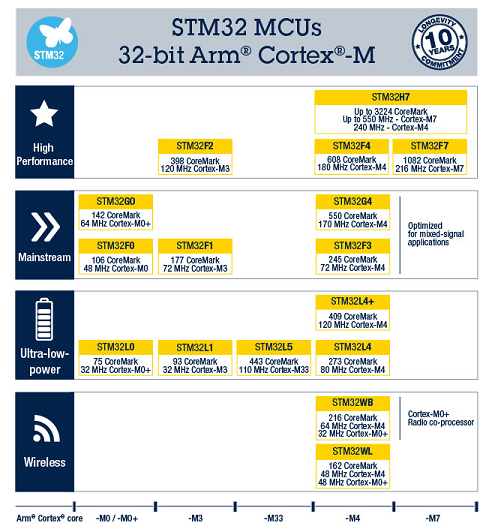
\includegraphics[width=0.7\linewidth]{img/przekroj_stm.png}
    \caption{Przekrój zastosowań mikrokontrolerów z rodziny STM32 \cite{b_site_STM32}}
    \label{f_przekroj_stm}
\end{figure}

Mikrokontrolery oferowane przez ST są szeroko wykorzystywane w zastosowaniach zarówno hobbystycznych, komercyjnych, jak i specjalistycznych. Posiadają duże wsparcie producenta, jak również wiele dedykowanych, stale rozwijanych i darmowych narzędzi ułatwiających pracę z nimi. Dokumentacja jest bardzo przejrzysta oraz ogólnodostępna na stronie producenta, zawiera pełny opis dostępnych peryferiów oraz ich specyfikację. Większość układów wspiera także FreeRTOS, co umożliwia wygodne użycie ich w~systemach czasu rzeczywistego.

Firma ST oferuje także płytki rozwoje z serii Nucleo i Discovery. Są one idealne jako pierwszy etap rozwoju projektu, ponieważ pozwalają korzystać z zalet mikrokontrolera zanim powstanie płytka drukowana, na której zostanie on umieszczony. Płytki rozwojowe pozwalają w ten sposób rozwijać projekt bez nadmiernych początkowych kosztów. Przykładem wykorzystania takiej płytki rozwojowej jest otrzymany przeze mnie prototyp sztucznej skóry widoczny na rysunku \ref{f_otrzymany_prototyp}, gdzie jako płytka rozwojowa zostało użyte Nucleo-F767ZI \cite{b_report_otrzymane}.
Dodatkowo narzędzia oferowane przez ST pozwalają przenosić napisany wcześniej kod na mikrokontrolery z innych serii co ułatwia przeniesienie pracy wykonanej na płytce rozwojowej na gotowy prototyp.

W kolejnych podrozdziałach zostały omówione niektóre z oferowanych przez ST narzędzi oraz szerokie wsparcie dla środowisk programistycznych, nie tylko tych promowanych przez ST. Narzędzia te pozwalają na dużo łatwiejszą pracę z mikrokontrolerem.

\subsubsection{Biblioteka HAL}
Jednym z narzędzi ułatwiających pracę była wykorzystana przeze mnie biblioteka HAL. Biblioteka ta jest oficjalnie dystrybuowana przez ST jako podstawowa biblioteka umożliwiająca i ułatwiająca programowanie mikrokontrolerów STM32. W praktyce biblioteka ta jest wysokopoziomowym interfejsem do części sprzętowej mikrokontrolera, pozwalając programiście w łatwy i przystępny sposób programować mikrokontroler.
Należy jednak pamiętać, że biblioteka wysokopoziomowa HAL poświęca jednak część wydajności i~szybkości działania mikrokontrolera na rzecz łatwości programowania i uniwersalności napisanego kodu.

Biblioteka HAL pozwala użytkownikowi także na wygodne przenoszenie kodu pomiędzy mikrokontrolerami z różnych rodzin STM32. Wygodne przenoszenie kodu pozwala na zmianę mikrokontrolera nawet na zaawansowanym etapie pracy, kiedy okaże się, że~obecna konfiguracja jest niewystarczająca. 
Jest to możliwe dzięki implementacji publicznych funkcji wykorzystywanych przez użytkownika w sposób dedykowany dla danego mikrokontrolera, przy czym z perspektywy użytkownika sposób wywołania funkcji (nazwa, parametry wywołania) się nie zmieniają. Takie podejście jest głównym powodem, dla którego napisany program sterownika sztucznej skóry korzystał z tej biblioteki.

\subsubsection{Narzędzie STM32CubeMX}
STM32CubeMX jest bardzo przydatnym narzędziem dystrybuowanym oficjalnie przez ST Microelectronics. Na etapie projektowania systemu, w szczególności części elektronicznej, pozwala na ułatwienie doboru odpowiedniego mikrokontrolera i przypisanie pinów mikrokontrolera do pracy z dobranymi układami. Na etapie programowania rozwiązanie umożliwia wygodną konfigurację używanego mikrokontrolera oraz wstępne wygenerowanie kodu poprawnie inicjującego wszystkie niezbędne do pracy peryferia.

Dobór mikrokontrolera polega na wybraniu najlepszego układu do danego rozwiązania. Nie jest to łatwe, ponieważ na rynku jest nawet po kilkaset różnych konfiguracji mikrokontrolerów od wielu producentów. Dlatego wiele firm, w tym ST, udostępnia narzędzie do wyboru odpowiedniego układu, poprzez filtrowanie całej bazy na podstawie wprowadzonych wymaganych parametrów. Takie narzędzie filtrowania zostało zaimplementowane właśnie w narzędziu STM32CubeMX. Wymogi w moim przypadku nie były bardzo ograniczające, więc mój wybór padł na prosty i tani mikrokontroler STM32F103RB, którego wcześniej już używałem w innych projektach. Ekran doboru mikrokontrolera jest widoczny na rysunku \ref{f_cube_micro}.

\begin{figure}[!h]
    \centering
    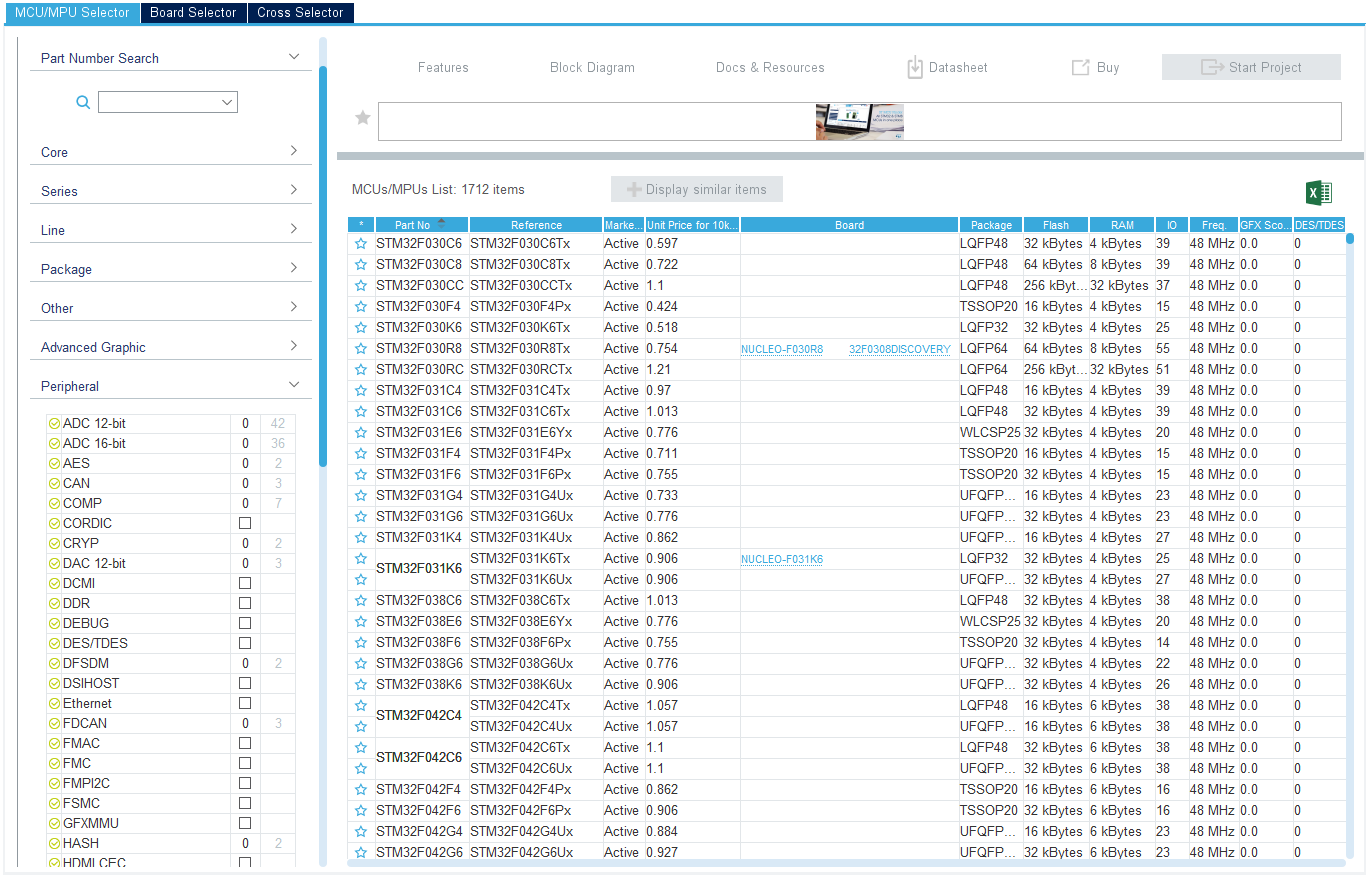
\includegraphics[width=0.95\linewidth]{img/cube_mcu_select.png} 
    \caption{Okno wyboru mikrokontrolera programu STM32CubeMX} 
    \label{f_cube_micro}
\end{figure}

Po wyborze odpowiedniego mikrokontrolera narzędzie przechodzi do widoku konfiguracji peryferiów. Widok ten przedstawia podgląd mikrokontrolera i wyprowadzonych z niego pinów wraz z oznaczeniem ich przeznaczenia i tego, czy są używane czy wolne. Na tym etapie można skonfigurować wybrane peryferia, a program automatycznie zarezerwuje potrzebne do tego piny i odświeży podgląd mikrokontrolera. W przypadku wystąpienia konfliktu lub braku możliwości użycia danego peryferium program nie pozwoli nam go skonfigurować. Narzędzie umożliwia także ręczną konfigurację pinów mikrokontrolera lub przenoszenie miejsca wyprowadzenia danego peryferium spośród możliwości oferowanych przez mikrokontroler.

Rozwiązanie z podglądem wyjść pinów mikrokontrolera jest bardzo przydatne na~etapie projektowania obwodu drukowanego do obsługi mikrokontrolera. Pozwala już na dość wczesnym etapie zaplanować wygląd i kształt takiej płytki. Taki widok pozwala także zaplanować, które wyjścia mikrokontrolera użyć, aby jak najmniejszym kosztem poprowadzić połączenia do dalszych komponentów na płytce. Bazując na własnym doświadczeniu, takie podejście znacznie zmniejsza możliwość wystąpienia błędu w porównaniu do metody alternatywnej planowania wyprowadzeń, czyli samej dokumentacji. Dokumentacja również zawiera wszystkie potrzebne informacje, lecz jej forma (tekst i~tabele) nie jest w stanie wykryć wykonanych przez projektanta błędów. CubeMX pozwala dodatkowo na wygodne ustawianie częstotliwości taktowania poszczególnych peryferiów. Podczas doboru częstotliwości taktowania obliczane i korygowane są częstotliwości taktowania innych peryferiów zależne od tej modyfikowanej przez użytkownika. Pozwala to na~znaczne zmniejszenie ilości błędów związanych z błędną częstotliwością taktowania na poszczególnych peryferiach. Wygląd programu w oknie konfiguracji mikrokontrolera został przestawiony na rysunku \ref{f_cube_konf}.

\begin{figure}[!h]
    \centering
    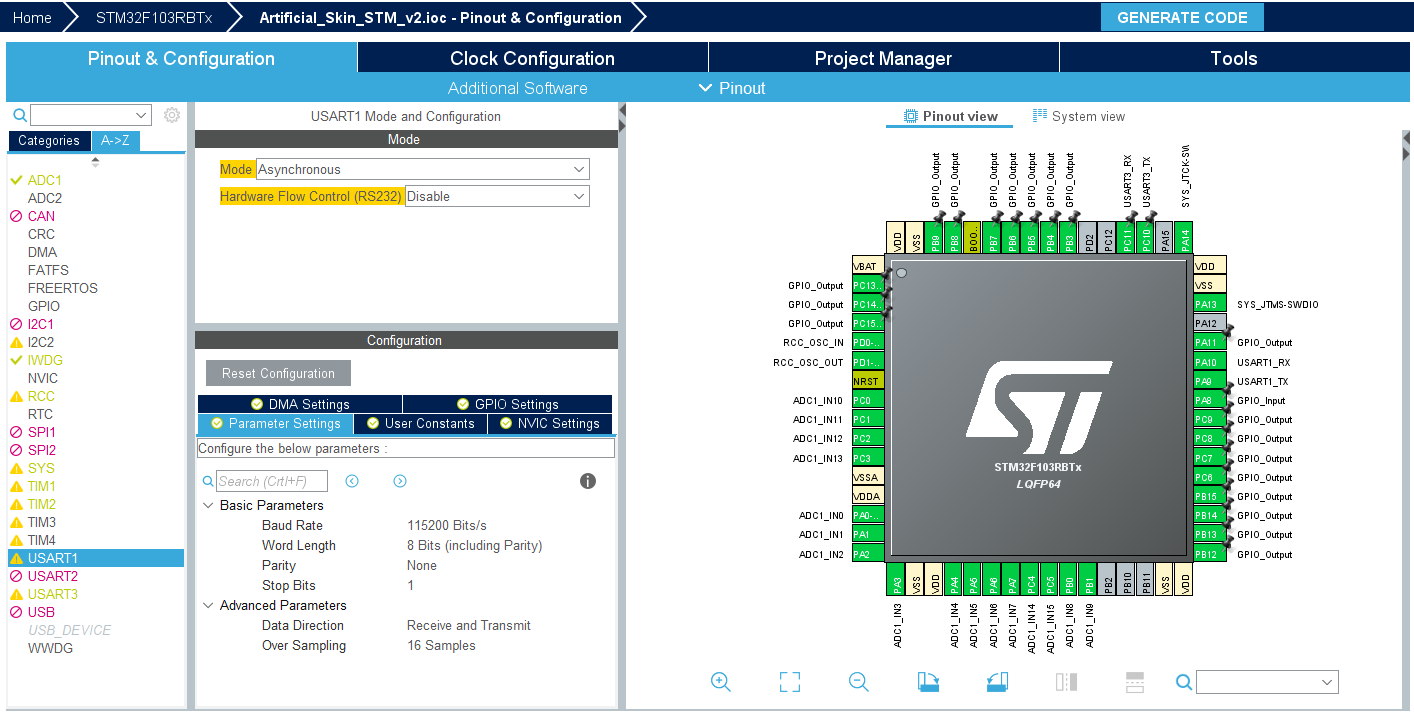
\includegraphics[width=0.95\linewidth]{img/cube_config.png}
    \caption{Okno konfiguracji mikrokontrolera programu STM32CubeMX} 

  \label{f_cube_konf}
\end{figure}

Ostatnią, ale nie mniej ważną funkcją tego narzędzia jest generowanie kodu źródłowego programu. Wygenerowany kod źródłowy jest od razu gotowy do skompilowania i działania. Co prawda taki kod jeszcze nie wykonuje oczekiwanego przez programistę zadania, ale pozwala na ominięcie żmudnej pracy uruchamiania wszystkich peryferiów ręcznie. Wygenerowany kod jest logicznie podzielony na pliki w zależności od peryferium. Niestety jest on również nieprzejrzysty, więc jego uporządkowanie wymaga od programisty trochę pracy \cite{b_site_cube}.

\subsubsection{Środowisko programistyczne CLion}
Po wygenerowaniu wstępnego kodu źródłowego potrzebne jest jego uzupełnienie o~zaplanowane funkcje. Na rynku do wyboru jest wiele różnych środowisk programistycznych, ale mój wybór padł na środowisko, które wspiera programowanie mikrokontrolerów STM32. Wybrane zostało środowisko oferowane przez JetBrains - CLion, które od wersji 2019.1 oficjalnie posiada dedykowane wsparcie dla mikrokontrolerów z~rodziny STM32 \cite{b_site_CLion_STM_support}. Wcześniejsze wersje oprogramowania wspierały tylko z wykorzystaniem odpowiednich dodatkowo instalowanych wtyczek \cite{b_site_CLion_STM_support_v2}. % Co działało dużo lepiej, ale już chuj z tym
Wsparcie środowiska dla systemów STM32 objawia się przede wszystkim poprzez wbudowaną funkcję do generacji pliku \textit{CMakeLists.txt} niezbędnego, aby w środowisku CLion poprawnie skompilować projekt. Generacja tego pliku jest opierana na wygenerowanych wcześniej przez program STM32CubeMX plikach, zawierających wszystkie informacje o docelowym mikrokontrolerze.
Wspierany jest także zautomatyzowany wybór mikrokontrolera docelowego, na który program będzie wgrywany, spośród dostępnych w bibliotekach list. Po wykonaniu tych dwóch kroków środowisko jest skonfigurowane i gotowe do kompilacji oraz wgrywania programu na mikrokontroler \cite{b_site_CLion_STM_support}.

Środowisko CLion wspiera także debugowanie napisanych programów i nie potrzebuje do tego specjalistycznych urządzeń dostarczanych przez ST. Do debugowania (jak również zwykłego programowania) wystarczy posiadać konwerter na interfejs SWD. Debugowanie mikrokontrolerów, podobnie jak zwykłych programów, polega na zatrzymaniu programu po osiągnięciu oznaczonego miejsca w kodzie programu i zatrzymaniu programu w tym miejscu. Po zatrzymaniu można przeglądać jakie program przyjmuje wartości dla użytych zmiennych lub samemu nadawać tym zmiennym wartości. Debugowanie mikrokontrolerów różni się od debugowania zwykłych programów tym, że mikrokontroler jest w~stanie pracować na przerwaniach. W kodzie programu objawia się to faktem używania funkcji, do których kod nie ma odniesień. Należy to mieć na uwadze, ponieważ pomiędzy podglądaniem zmiennych program może zmieniać ich wartości właśnie w przerwaniach bez naszej wiedzy. 
Ograniczenia jakie występują w środowisku polegają na tym, że CLion nie pozwala na debugowanie z oznaczeniem wielu miejsc w kodzie, w których program się zatrzyma.

Opisane w powyższych akapitach cechy zawiera praktycznie każde środowisko przystosowane do programowania mikrokontrolerów. To, w czym CLion zdobywa przewagę nad innymi środowiskami to wygoda użytkowania. Na tę wygodę składają się między innymi: ciemny motyw (nie każde środowisko taki posiada% tak o tobie myślę Eclipse
), intuicyjny interfejs, duża dowolność w konfiguracji środowiska. Program posiada także sporo skrótów klawiaturowych przyspieszających pracę oraz inne przydatne funkcjonalności jak np. zakładki do konkretnych miejsc w kodzie. Z tych właśnie powodów, i częściowo z przyzwyczajenia do środowiska, mój wybór padł właśnie na CLiona.

% STMStudio, StLinkUtility??

% Opisywać Altiuma?

% \subsection{Obsługa portów komunikacyjnych - PuTTY}
% Jak mi się będzie nudziło to napiszę to jako zapychacz

\subsection{Środowisko pracy - ROS}

System ROS (Robot Operating System) jest potężnym i elastycznym środowiskiem pozwalającym na tworzenie i testowanie oprogramowania robotów. Zawiera wiele narzędzi i bibliotek dostosowanych specjalnie do pracy w tak specjalistycznym jak robotyka zakresie. ROS jest również systemem pozwalającym na połączenie różnych modułów percepcyjnych i aktuatorów w jednym systemie \cite{b_site_ROS}.

ROS jest strukturalnie podzielony na węzły odpowiadające uruchomionym procesom, tematy odpowiadające kanałom przesyłania danych, usługi będące węzłami wykonującymi pojedyncze akcje oraz serwery parametrów przechowujących informacje, które nie zmieniają się zbyt często. Jeden węzeł może wysyłać i odbierać na wielu tematach, podobnie jak na jeden temat może nadawać wiele węzłów. Tematy mogą być także pogrupowane w zależności od tego, z jakiem pakietem są związane. Cała ta nieskomplikowana w założeniach struktura jest otwarta na modyfikacje i rozbudowę poprzez dodawanie kolejnych węzłów \cite{b_site_ROS_wiki}.

Narzędzia udostępniane przez ROS są bardzo pomocne w pracach, szczególnie na~etapie testowania rozwiązań i szukania błędów w implementacji. Dostępnych narzędzi jest wiele, ale jednym z najważniejszych jest RVIZ. RVIZ jest narzędziem służącym do wizualizacji aktualnego stanu robota w przestrzeni trójwymiarowej. Nie jest to jednak symulator, ponieważ potrafi on pokazywać tylko informacje znane robotowi, które może on odczytać wykorzystując zamocowane na nim czujniki lub kamery. Widoczne są także informacje zapisane wcześniej do pamięci robota, takie jak mapa terenu \cite{b_site_ROS_tools}. Widok narzędzia RVIZ z odwzorowaną mapą laboratorium został przedstawiony na rysunku \ref{f_ros_tools_rviz}.

\begin{figure}[!h]
    \centering
    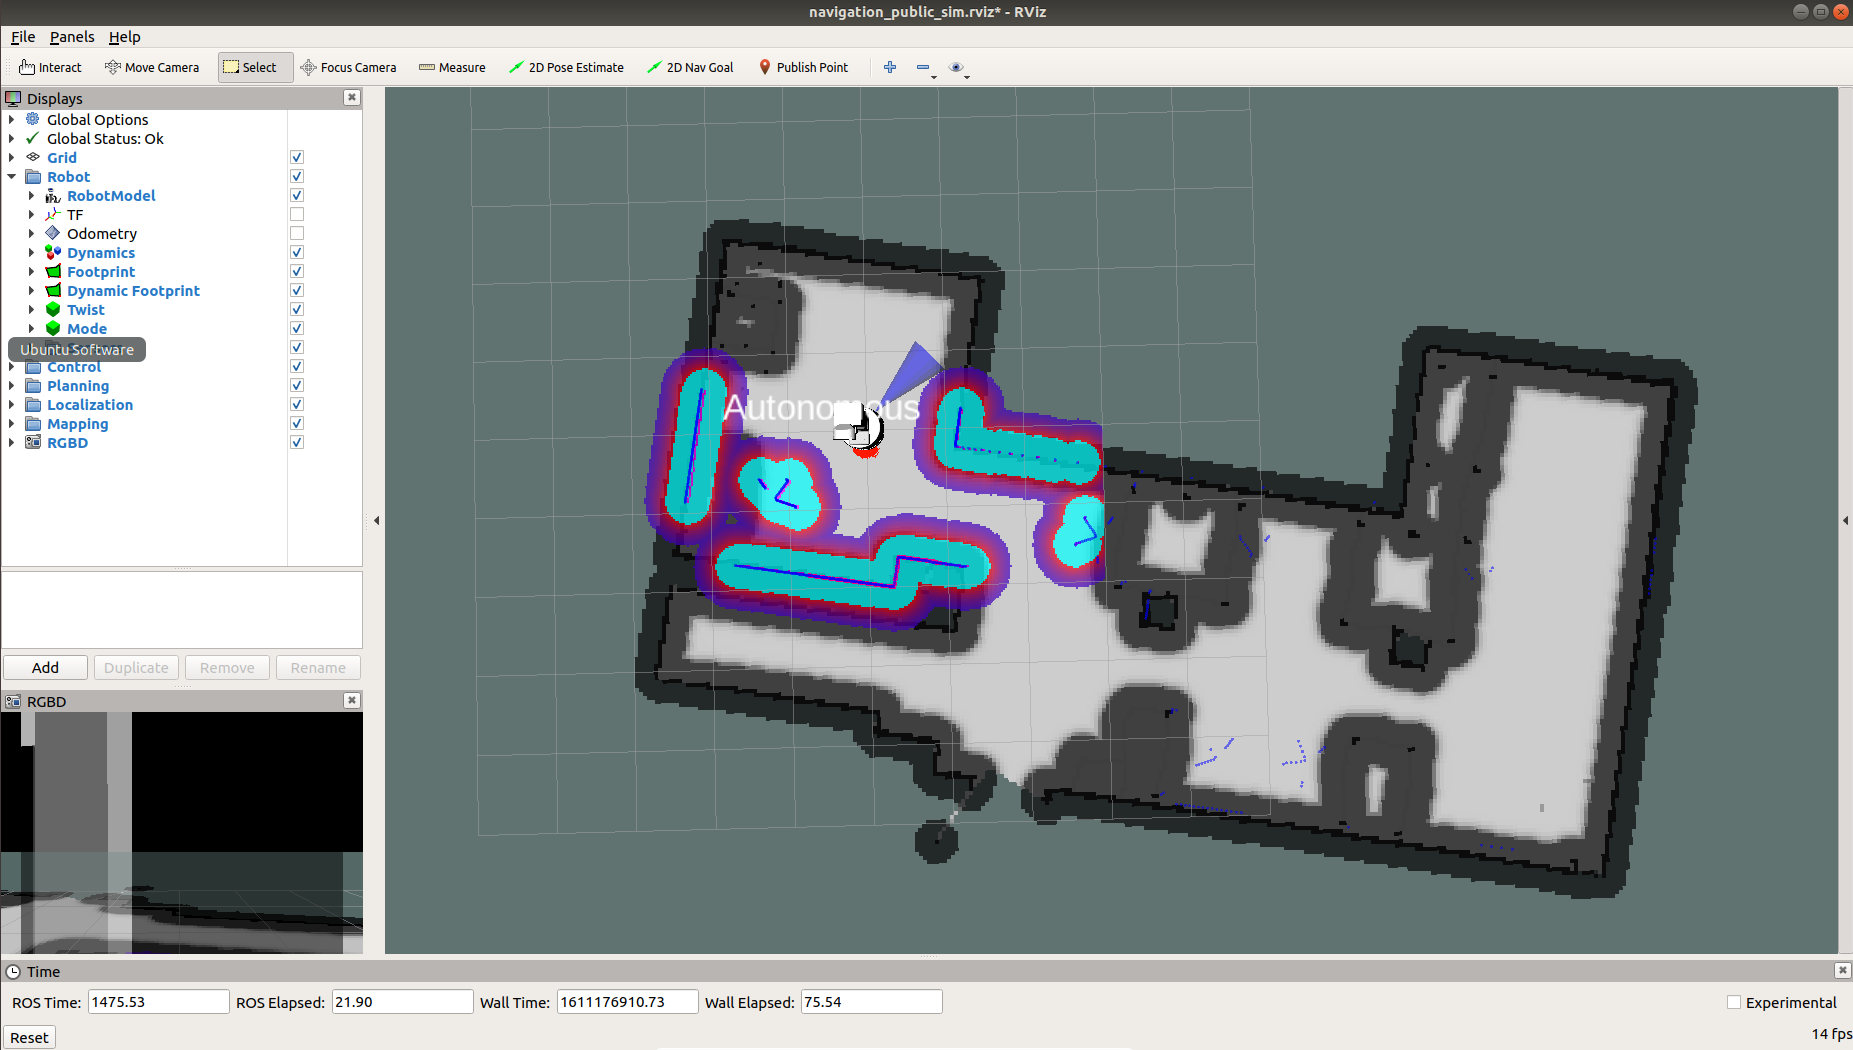
\includegraphics[width=0.95\linewidth]{img/ros_tools_rviz.png} 
    \caption{Narzędzie RVIZ \cite{b_site_ROS_tools}} 
     \label{f_ros_tools_rviz}
    % \vspace{4ex}
    \end{figure}

Kolejnym narzędziem znacząco pomagającym w podglądzie aktualnego stanu robota jest rqt\_graph. Rqt\_graph wizualizuje aktualny stan robota pokazując strukturę węzłów i~tematy, które znajdują się w całej strukturze systemu. Narzędzie to wizualizuje strukturę przedstawiając ją w formie grafu skierowanego. Udostępnione są też dodatkowe funkcje odfiltrowania niektórych danych, np. węzłów, które nie publikują danych i nie wpływają w żaden sposób na pracę systemu \cite{b_site_ROS_tools}. Przykładowy widok narzędzia rqt\_graph jest widoczny na rysunku \ref{f_ros_tools_rqt}.


    \begin{figure}[!h]
    
    \centering
    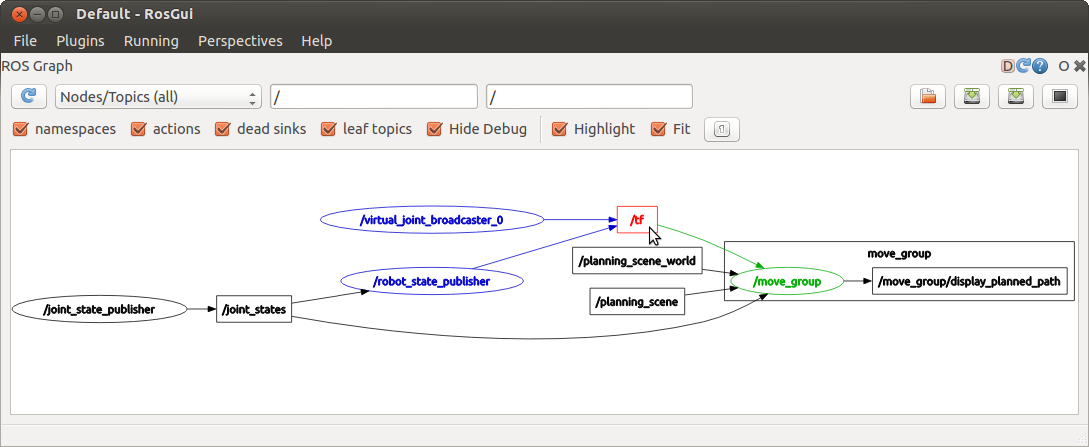
\includegraphics[width=0.95\linewidth]{img/ros_tools_rqt.png}
    \caption{Narzędzie Rqt\_graph \cite{b_site_ROS_tools}} 
     \label{f_ros_tools_rqt}
    % \vspace{4ex}

\end{figure}

% plot 

ROS oferuje także narzędzia opierające się głównie na komunikacji za pomocą konsoli, a jednym z częściej używanych jest rostopic. Rostopic daje duże możliwości w kontrolowaniu tematów (kanałów danych). Najczęściej wykorzystywana jest funkcja echo, która wyświetla na konsoli, w czasie rzeczywistym, wszystkie informacje, które są przesyłane danym strumieniem. Pozwala to na szybkie znajdowanie i naprawianie błędów, jeśli przesyłane są złe informacje lub w ogóle nie są przesyłane. Rostopic pozwala także na wysyłanie wiadomości na podany przez operatora temat. Dodatkowo umożliwia także otrzymywanie informacji o wszystkich dostępnych w systemie tematach i typie informacji na nich wysyłanych \cite{b_site_ROS_tools}.

Innymi przydatnymi narzędziami są rosbag oraz rqt\_bag pozwalające na zbieranie i~przeglądanie zebranych danych. Rosbag jest narzędziem przeznaczonym do zbierania danych przesyłanych na tematach oraz ich późniejszego odtworzenia, a nawet wysłanie z powrotem na temat. Rqt\_bag jest podobnym narzędziem do rosbag, ale posiada wbudowany interfejs użytkownika \cite{b_site_ROS_tools}.


\subsection{Platforma symulacyjna - Gazebo}
\label{ss_narzedzia_gazebo}
Ważną kwestią, jeśli chodzi o testowanie, jest przeprowadzenie wstępnych testów na symulacji. Używanie symulacji w testowaniu robotów jest ważne, aby w żaden sposób nie narażać człowieka, robota ani środowiska na jakiekolwiek niebezpieczeństwa. 
Symulator dostępny jest także lokalnie na komputerze bez potrzeby prowadzenia testów w laboratorium, co znacznie ułatwiło mi testy szczególnie w czasie pandemii. 
Finalnie jednak w ten sposób nie można sprawdzić działania prototypu w rzeczywistych warunkach i~zweryfikować czy współpracuje on z fizycznym robotem.

Środowisko symulacyjne doskonale sprawdziło się natomiast do celów weryfikacji wybranych i zaimplementowanych algorytmów sterowania robotem. Można sprawdzić czy robot się prawidłowo zachowuje i reaguje na wysyłane sygnały.
W niniejszym przypadku symulacja pozwoliła także w wygodny sposób skonfigurować dołączany do systemu węzeł bez ryzyka uszkodzenia sprzętu. Sprawdzona została także poprawność działania zaprojektowanej sztucznej skóry i sprawność komunikacji sterownika z komputerem.

W kwestii symulatora wybór padł na program Gazebo, który jest bardzo dobrze przystosowany do integracji z systemem ROS i był projektowany z myślą o testowaniu robotów. Gazebo posiada bardzo wygodny interfejs, dobrą fizykę i pozwala użytkownikowi na bardzo dużą swobodę w projektowaniu jego elementów. Gazebo wspiera także dużą liczbę różnych czujników, efektorów i innych podzespołów, jak również roboty funkcjonujące na rynku \cite{b_site_Gazebo}.

Dla ułatwienia testów wykorzystane zostały istniejące i wykonane wcześniej przez zespół laboratoryjny pakiety: świata, który był dobrym odwzorowaniem faktycznego laboratorium oraz robota. Odwzorowanie robota było oparte na pakiecie, który udostępnia firma go produkująca - PAL Robotics. Pozwoliło mi to na testy w praktycznie tym samym środowisku, co prowadzone później testy fizyczne.

\subsection{Platforma testowa - robot Tiago}

Robot Tiago jest produkowany przez hiszpańską firmę PAL Robotics, która ma w~swoim portfolio jeszcze kilka robotów do innych zastosowań (w tym przemysłowych). Zaprojektowany przez nich robot Tiago jest typowym robotem asystującym mającym za zadanie współpracować z ludźmi w ich domowym środowisku i wykonywać zlecone mu zadania \cite{b_site_tiago}.

Tiago jest robotem modułowym, co znaczy że można dopasowywać jego możliwości i zainstalowane podzespoły do własnych potrzeb. Jako podstawa oferowana jest baza jezdna z komputerem, czujnikami odległości oraz kamerą stereo. Jako dodatkowe opcje można wybrać manipulatory o siedmiu stopniach swobody, ich chwytaki, dodatkowy osprzęt (kamery, tablet), czy też wydajniejsze podzespoły wewnętrzne robota \cite{b_site_tiago}. Sam robot został przedstawiony na rysunku \ref{f_tiago_zwykly}.

Robot wyposażony jest przede wszystkim w układ sterowania wykorzystujący możliwości procesorów Intel\textsuperscript{\textregistered}Core\texttrademark i5 lub i7, co zapewnia mu dużą moc obliczeniową. Każda wersja posiada także laserowy czujnik odległości zamontowany z przodu w podstawie robota. Czujnik laserowy ma zasięg zależnie od wersji od $5,6m$ do $25m$ zasięgu i pole widzenia $\ang{220}$. U podstawy znajduje się napęd w standardowej konfiguracji układu różnicowego, czyli dwa koła niezależnie napędzane oraz kilka swobodnych, służących przede wszystkim jako punkty podparcia. W górnej części robota, która przypomina głowę, umieszczona została kamera stereowizyjna, która pozwala na wykorzystywanie na robocie zaawansowanych algorytmów przetwarzania obrazu. Niedaleko znajduje się także mikrofon rejestrujący dźwięki z otoczenia. Cała górna część umieszczona została na podnoszonym i~opuszczanym przez robota tułowiu. Robot posiada także wbudowaną komunikację WiFi, co umożliwia w pełni bezprzewodowe sterowanie nim, również przez Internet. Komunikacja ta upraszcza również użycie robota w coraz bardziej popularnych systemach IOT \cite{b_site_tiago}.

PAL Robotics udostępnia także za darmo poradniki jak używać ich robota i modelu ich robota w systemie ROS. Oferują oni pełne wsparcie opisanych wcześniej rozwiązań co znacznie ułatwia wstępne testowanie kodu, nawet bez dostępu do samego robota. Oferowane przez nich narzędzia posiadają także funkcję dostosowywania osprzętu robota według własnych upodobań \cite{b_site_tiago, b_site_tiago_ROS}.
